\documentclass[aspectratio=169]{beamer}

\usepackage{Archivo}
\renewcommand{\sfdefault}{\rmdefault}
\usepackage{graphicx}
\usepackage{tikz}
\usetikzlibrary{calc,positioning}
\tikzset{
  invisible/.style={opacity=0, text opacity=0},
  visible on/.style={alt={#1{}{invisible}}},
  alt/.code args={<#1>#2#3}{%
    \alt<#1>{\pgfkeysalso{#2}}{\pgfkeysalso{#3}}%
  },
}
\usepackage[most]{tcolorbox}
\usepackage{listings}

%% ---- Superteam Poland brand colors ----
\definecolor{stpldark}{HTML}{0B0E0F}   % near-black background
\definecolor{stplcard}{HTML}{161A1B}   % card / block surface
\definecolor{stplborder}{HTML}{1E2526}  % subtle track color for progress bar
\definecolor{stplred}{HTML}{DC143C}    % brand crimson red
\definecolor{stplwhite}{HTML}{FFFFFF}  % white
\definecolor{stplmuted}{HTML}{8A9BA8}  % muted / secondary text

\usetheme{default}
\setbeamersize{text margin left=0.85cm, text margin right=0.85cm}

%% ---- Background & base text ----
\setbeamercolor{background canvas}{bg=stpldark}
\setbeamercolor{normal text}{fg=stplwhite, bg=stpldark}
\usebeamercolor{normal text}

%% ---- Background image helpers ----
\newcommand{\stpldefaultbg}{%
  \setbeamertemplate{background}{%
    \begin{tikzpicture}[remember picture, overlay]
      \node[at=(current page.center), inner sep=0pt] {%
        \includegraphics[width=\paperwidth,height=\paperheight]{images/bg-default.png}%
      };
      \fill[stplborder]
        (current page.north west) rectangle
        ([yshift=-2.5pt]current page.north east);
      \pgfmathsetmacro{\stplprog}{\insertframenumber/\inserttotalframenumber}
      \fill[stplred]
        (current page.north west) rectangle
        ($(current page.north west)+(\stplprog\paperwidth,-2.5pt)$);
    \end{tikzpicture}%
  }%
}
\newcommand{\stplherobg}{%
  \setbeamertemplate{background}{%
    \includegraphics[width=\paperwidth,height=\paperheight]{images/bg-hero.png}%
  }%
}
\stpldefaultbg

%% ---- Structure ----
\setbeamercolor{structure}{fg=stplred}

%% ---- Title slide metadata ----
\setbeamercolor{title}{fg=stplwhite}
\setbeamercolor{subtitle}{fg=stplred}
\setbeamercolor{author}{fg=stplwhite}
\setbeamercolor{institute}{fg=stplmuted}
\setbeamercolor{date}{fg=stplmuted}

%% ---- Frame title: flat, no box background ----
\setbeamercolor{frametitle}{fg=stplwhite, bg=}
\setbeamerfont{frametitle}{size=\large, series=\bfseries}
\setbeamertemplate{frametitle}{%
  \vspace{0.35cm}%
  {\centering\insertframetitle\par}%
  \nointerlineskip\vspace{0.18cm}%
  \hfil{\color{stplred}\rule{2.2cm}{1.5pt}}\hfil\par%
}



%% ---- Incremental reveals ----
%% Bullets reveal one at a time by default. See style.md §4.5 for the two
%% per-frame opt-outs (static frame: `\begin{frame}<1>{...}`; manually
%% choreographed frame: `\beamerdefaultoverlayspecification{}` at frame top).
\beamerdefaultoverlayspecification{<+->}

%% ---- Bullet items ----
\setbeamercolor{itemize item}{fg=stplred}
\setbeamercolor{itemize subitem}{fg=stplmuted}
\setbeamercolor{itemize subsubitem}{fg=stplmuted}
\setbeamertemplate{itemize item}{\bfseries\textendash}
\setbeamertemplate{itemize subitem}{\small\textendash}
\setbeamercolor{enumerate item}{fg=stplred}
\setbeamercolor{enumerate subitem}{fg=stplmuted}
\setbeamertemplate{enumerate item}{\textcolor{stplred}{\bfseries\insertenumlabel.}}
\setbeamertemplate{enumerate subitem}{\textcolor{stplmuted}{\small\insertenumlabel.}}

%% ---- Blocks (flat left-accent via tcolorbox) ----
\tcbset{
  stplbase/.style={
    enhanced, breakable,
    colback=stplcard, coltext=stplwhite,
    coltitle=stplwhite, fonttitle=\bfseries,
    boxrule=0pt, leftrule=3pt,
    arc=0pt, outer arc=0pt,
    top=5pt, bottom=5pt, left=7pt, right=7pt,
    toptitle=4pt, bottomtitle=4pt,
    titlerule=0pt,
  },
}
\renewenvironment{block}[1]{%
  \pause%
  \begin{tcolorbox}[stplbase, colframe=stplred, title={#1}]%
}{%
  \end{tcolorbox}%
}
\renewenvironment{alertblock}[1]{%
  \pause%
  \begin{tcolorbox}[stplbase, colframe=stplred!75!black,
    colback=stplred!10!stplcard, title={#1}]%
}{%
  \end{tcolorbox}%
}
\renewenvironment{exampleblock}[1]{%
  \pause%
  \begin{tcolorbox}[stplbase, colframe=stplmuted, title={#1}]%
}{%
  \end{tcolorbox}%
}

%% ---- Code listings (Rust + Anchor) ----
\lstdefinelanguage{Rust}{
  keywords={fn,pub,struct,impl,trait,let,mut,self,Self,match,return,for,in,
            if,else,enum,use,mod,as,where,Option,Result,Some,None,Ok,Err,
            u8,u16,u32,u64,i64,u128,bool,String,Vec,Pubkey,Context,msg,vec,
            Account,Signer,Program,System,has_one,init,payer,space,seeds,bump},
  morecomment=[l]{//},
  morestring=[b]",
  sensitive=true,
}
\lstset{
  basicstyle=\ttfamily\scriptsize\color{stplwhite},
  backgroundcolor=\color{stplcard},
  keywordstyle=\color{stplred}\bfseries,
  commentstyle=\color{stplmuted},
  stringstyle=\color{stplmuted},
  showstringspaces=false,
  keepspaces=true,
  columns=fixed,
  basewidth=0.46em,
  frame=leftline,
  framerule=2pt,
  rulecolor=\color{stplred},
  xleftmargin=0.6em,
  aboveskip=0.4em,
  belowskip=0.2em,
  language=Rust,
  escapeinside={(*@}{@*)},
}

%% ---- Code reveal card (line-synced to bullets) ----
%% A block-styled card WITHOUT the block's auto-\pause, so it is visible from
%% the current overlay and its code lines can reveal in step with the itemize
%% bullets via (*@\onslide<k->@*) markers. The listing drops its own
%% background/frame (style=reveal) so the solid card shows through instead of
%% the per-line background going ragged as lines are covered.
\newtcolorbox{codeblock}[1]{stplbase, colframe=stplred, title={#1}}
\lstdefinestyle{reveal}{backgroundcolor={}, frame=none, xleftmargin=0pt,
  aboveskip=0pt, belowskip=0pt}

%% ---- Table of contents ----
\setbeamercolor{section in toc}{fg=stplwhite}
\setbeamercolor{subsection in toc}{fg=stplmuted}
\setbeamertemplate{section in toc}{%
  {\color{stplred}\textbf{\textendash}}\hspace{0.5em}\inserttocsection%
}

%% ---- Footline: minimal ----
%% Transparent bg so the background image shows through (normal text has
%% bg=stpldark, which would paint a flat band over the image's bottom glow).
\setbeamercolor{footline}{fg=stplwhite, bg=}
\setbeamertemplate{footline}{%
  \begin{beamercolorbox}[wd=\paperwidth, ht=0pt, dp=0.55cm]{footline}%
    \hspace{0.85cm}%
    \raisebox{-0.42cm}{\includegraphics[height=0.42cm]{images/stpl-logo.png}}%
    \hfill%
    \raisebox{-0.24cm}{\textcolor{stplmuted}{\tiny\insertframenumber\,/\,\inserttotalframenumber}}%
    \hspace{0.85cm}%
  \end{beamercolorbox}%
}
\setbeamertemplate{navigation symbols}{}

%% ---- Title page defaults (decks may override) ----
\date{\the\year}

%% ---- Title frame helper (uses hero background) ----
\newcommand{\maketitleframe}{%
  \stplherobg
  \begin{frame}[plain]%
    \titlepage%
  \end{frame}%
  \stpldefaultbg
}

%% ---- Section divider slides ----
\AtBeginSection[]{%
  \stplherobg
  \begin{frame}[plain]
    \begin{tikzpicture}[remember picture, overlay]
      \fill[stplred, opacity=0.07]
        ([xshift=-2.5cm]current page.east) circle (5.5cm);
      \fill[stplred]
        (current page.north west) rectangle ([xshift=5pt]current page.south west);
    \end{tikzpicture}%
    \vfill
    \hspace{0.1\paperwidth}%
    \begin{minipage}{0.8\paperwidth}
      \textcolor{stplmuted}{\small Section \thesection}\\[0.35cm]
      {\color{stplwhite}\LARGE\bfseries\insertsectionhead}\\[0.25cm]
      {\color{stplred}\rule{3cm}{1.5pt}}
    \end{minipage}%
    \vfill
  \end{frame}%
  \stpldefaultbg
}

%% ---- Title page ----
\setbeamertemplate{title page}{%
  \begin{tikzpicture}[remember picture, overlay]
    \fill[stplred]
      (current page.north west) rectangle ([xshift=5pt]current page.south west);
    \fill[stplred, opacity=0.07]
      ([xshift=-3cm,yshift=3cm]current page.north east) circle (5.5cm);
    \fill[stplred, opacity=0.04]
      ([yshift=-1.5cm]current page.south east) circle (3.5cm);
  \end{tikzpicture}%
  \vfill
  \hspace{0.08\paperwidth}%
  \begin{minipage}{0.85\paperwidth}
    \includegraphics[width=3cm]{images/stpl-logo.png}\par
    \vspace{0.8cm}
    {\usebeamerfont{title}\usebeamercolor[fg]{title}\inserttitle}\par
    \vspace{0.2cm}
    {\color{stplred}\rule{3cm}{1.5pt}}\par
    \vspace{0.3cm}
    {\usebeamerfont{subtitle}\usebeamercolor[fg]{subtitle}\insertsubtitle}\par
    \vspace{0.65cm}
    {\usebeamerfont{author}\usebeamercolor[fg]{author}\insertauthor}\par
    \vspace{0.12cm}
    {\small\textcolor{stplmuted}{\insertinstitute\enspace·\enspace\insertdate}}
  \end{minipage}%
  \vfill
}


\usepackage[utf8]{inputenc}
\usepackage[T1]{fontenc}

%% Deck-local listing keywords: the shared Anchor set in preamble.tex predates
%% the token-interface types used from Lekcja 9 onwards.
\lstset{morekeywords={Interface,InterfaceAccount,TokenInterface,TokenAccount,
                      Mint,Token,token,mint,authority,token_program,decimals,
                      derive,Accounts,InitSpace}}

\title{Tokeny}
\subtitle{Mint, konto tokenowe i Token-2022 --- Solana Bootcamp}
\author{}
\institute{Superteam Poland}

\begin{document}

\maketitleframe

\begin{frame}{Plan}
  \tableofcontents
\end{frame}

% ================================================================
\section{Czym jest token}

% 1. Wracamy do tokena --- problem hook (alertblock: gdzie mieszka saldo?)
\begin{frame}{Wracamy do tokena}
  \begin{itemize}
    \item Z Lekcji 2: token to \textbf{saldo z regułami} zaszytymi w kodzie
    \item Z Lekcji 5: wszystko na Solanie jest kontem --- więc saldo też
    \item Phantom pokazuje listę tokenów, a Lekcja 8 mówiła o \emph{mincie}
  \end{itemize}
  \vspace{0.25cm}
  \begin{alertblock}{Pytanie}
    Konto portfela ma adres i lamporty --- ani jednego pola na tokeny.
    Które konto trzyma saldo USDC?
  \end{alertblock}
\end{frame}

% 2. Mint --- term debut (block: def)
\begin{frame}{Mint}
  \begin{itemize}
    \item Definicja waluty mieszka w osobnym koncie --- to \textbf{Mint}
    \item Jedno konto opisuje walutę: podaż, precyzję i prawo do dodruku
    \item Kto trzyma \texttt{mint\_authority}, ten zwiększa podaż w dowolnej chwili
    \item Adres mintu jest identyfikatorem tokena --- USDC to konkretny adres
  \end{itemize}
  \vspace{0.15cm}
  \begin{center}
    
\begin{tikzpicture}[
        every node/.style={font=\scriptsize\bfseries, align=center},
        fld/.style={
          draw=stplred, line width=0.9pt,
          fill=stplcard, text=stplwhite,
          rounded corners=2pt,
          minimum width=2.6cm, minimum height=0.75cm, align=center,
        },
        lbl/.style={font=\tiny\itshape, text=stplmuted},
      ]
      \node[lbl] (t) at (-2.3, 0) {konto \textsc{Mint}};
      \node[fld] (a) at (0.2, 0) {supply\\[-1pt]\tiny\mdseries 21\,000\,000};
      \node[fld] (b) at (3.0, 0) {decimals\\[-1pt]\tiny\mdseries 6};
      \node[fld] (c) at (5.8, 0) {mint\_authority\\[-1pt]\tiny\mdseries klucz emitenta};
    \end{tikzpicture}
  \end{center}
  \vspace{0.15cm}
  \begin{block}{Definicja}
    Mint opisuje token, nie właściciela. Nie trzyma niczyjego salda ---
    to dowód osobisty waluty, nie portfel.
  \end{block}
\end{frame}

% 3. Konto tokenowe --- term debut (block: def)
\begin{frame}{Konto tokenowe}
  \begin{itemize}
    \item Saldo mieszka w jeszcze innym koncie --- to \textbf{Token Account}
    \item Wiąże trzy rzeczy: walutę, właściciela i kwotę
    \item Jedna para właściciel--mint to jedno konto tokenowe
    \item Konto tokenowe ma własny adres --- inny niż adres portfela
  \end{itemize}
  \vspace{0.15cm}
  \begin{center}
    
\begin{tikzpicture}[
        every node/.style={font=\scriptsize\bfseries, align=center},
        fld/.style={
          draw=stplred, line width=0.9pt,
          fill=stplcard, text=stplwhite,
          rounded corners=2pt,
          minimum width=2.6cm, minimum height=0.75cm, align=center,
        },
        lbl/.style={font=\tiny\itshape, text=stplmuted},
      ]
      \node[lbl] (t) at (-2.6, 0) {konto \textsc{Token Account}};
      \node[fld] (a) at (0.2, 0) {mint\\[-1pt]\tiny\mdseries która waluta};
      \node[fld] (b) at (3.0, 0) {owner\\[-1pt]\tiny\mdseries czyje saldo};
      \node[fld] (c) at (5.8, 0) {amount\\[-1pt]\tiny\mdseries ile jednostek};
    \end{tikzpicture}
  \end{center}
  \vspace{0.15cm}
  \begin{block}{Definicja}
    Saldo to nie pole portfela, tylko osobne konto, które na portfel wskazuje.
    Jeden portfel może mieć ich setki --- po jednym na każdy token.
  \end{block}
\end{frame}

% 4. Dwa konta --- static diagram frame (§4.5a: no synchronized bullets)
\begin{frame}<1>{Dwa konta}
  \vspace{0.1cm}
  \begin{center}
    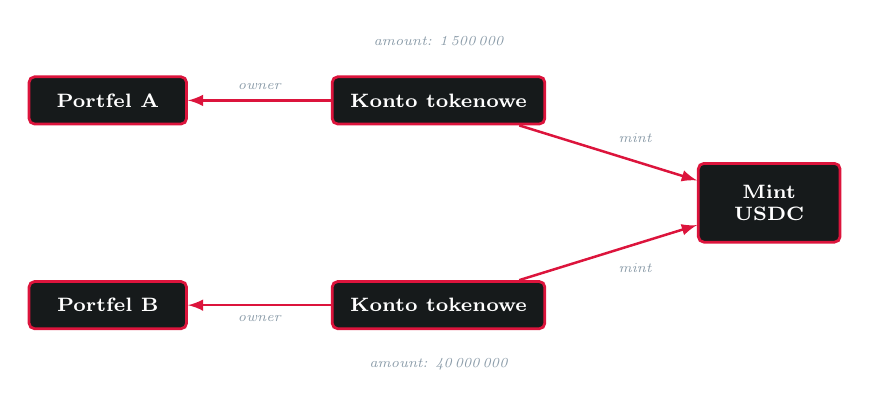
\begin{tikzpicture}[
        every node/.style={font=\scriptsize\bfseries, align=center},
        box/.style={
          draw=stplred, line width=1pt,
          fill=stplcard, text=stplwhite,
          rounded corners=2pt,
          minimum width=2.0cm, minimum height=0.6cm, align=center,
        },
        arr/.style={-latex, draw=stplred, line width=0.9pt},
        lbl/.style={font=\tiny\itshape, text=stplmuted},
      ]
      \node[box] (pa) at (0,  1.3) {Portfel A};
      \node[box] (pb) at (0, -1.3) {Portfel B};

      \node[box, minimum width=2.7cm] (ka) at (4.2,  1.3) {Konto tokenowe};
      \node[box, minimum width=2.7cm] (kb) at (4.2, -1.3) {Konto tokenowe};

      \node[box, minimum width=1.8cm, minimum height=1.0cm] (m) at (8.4, 0) {Mint\\USDC};

      \draw[arr] (ka) -- (pa) node[midway, above, lbl] {owner};
      \draw[arr] (kb) -- (pb) node[midway, below, lbl] {owner};
      \draw[arr] (ka) -- (m)  node[midway, above right, lbl] {mint};
      \draw[arr] (kb) -- (m)  node[midway, below right, lbl] {mint};

      \node[lbl] at (4.2,  2.05) {amount: 1\,500\,000};
      \node[lbl] at (4.2, -2.05) {amount: 40\,000\,000};
    \end{tikzpicture}
  \end{center}
  \vspace{0.15cm}
  \begin{itemize}
    % Static frame renders overlay 1 only --- the default <+-> would push the
    % second bullet to an overlay that never gets drawn.
    \item<1-> Jeden mint, dwa konta tokenowe --- dwa niezależne salda
    \item<1-> Saldo znajduje się po stronie konta, nie po stronie portfela
  \end{itemize}
\end{frame}

% 5. Miejsca po przecinku --- (exampleblock: worked example)
\begin{frame}{Miejsca po przecinku}
  \begin{itemize}
    \item Pole \texttt{amount} to liczba całkowita \texttt{u64} --- bez ułamków
    \item Mint ustala \texttt{decimals} i dopiero to przesuwa przecinek
    \item Sieć liczy wyłącznie na jednostkach bazowych, nigdy na ułamkach
    \item Instrukcja przelewu podaje \texttt{decimals} osobno --- sieć je weryfikuje
  \end{itemize}
  \vspace{0.1cm}
  \begin{center}
    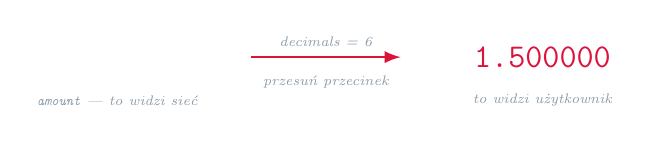
\begin{tikzpicture}[
        arr/.style={-latex, draw=stplred, line width=1pt},
        lbl/.style={font=\tiny\itshape, text=stplmuted},
      ]
      \node[font=\ttfamily\large, text=stplwhite] (raw) at (0, 0) {1\,500\,000};
      \node[lbl] at (0, -0.55) {\texttt{amount} --- to widzi sieć};

      \draw[arr] (1.7, 0) -- (3.6, 0)
        node[midway, above, lbl] {decimals = 6};
      \node[lbl] at (2.65, -0.32) {przesuń przecinek};

      \node[font=\ttfamily\large, text=stplred] (val) at (5.4, 0) {1.500000};
      \node[lbl] at (5.4, -0.55) {to widzi użytkownik};
    \end{tikzpicture}
  \end{center}
  \vspace{0.1cm}
  \begin{exampleblock}{Przykład}
    Pomyłka o jedno miejsce to pomyłka o dziesięciokrotność kwoty.
  \end{exampleblock}
\end{frame}

% ================================================================
\section{Adres konta tokenowego}

% 6. ATA --- term debut (block: def)
\begin{frame}{ATA}
  \begin{itemize}
    \item Każda para właściciel--mint potrzebuje swojego konta tokenowego
    \item Adres nie jest losowany --- wylicza się go z właściciela i mintu
    \item Takie kanoniczne konto to \textbf{Associated Token Account (ATA)}
    \item Portfel i eksplorator szukają salda dokładnie pod tym adresem
  \end{itemize}
  \vspace{0.1cm}
  \begin{center}
    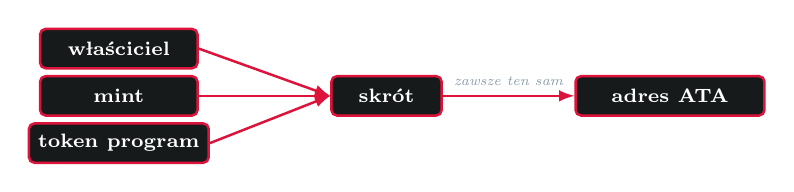
\begin{tikzpicture}[
        every node/.style={font=\scriptsize\bfseries, align=center},
        box/.style={
          draw=stplred, line width=0.9pt,
          fill=stplcard, text=stplwhite,
          rounded corners=2pt,
          minimum width=2.0cm, minimum height=0.5cm, align=center,
        },
        arr/.style={-latex, draw=stplred, line width=0.9pt},
        lbl/.style={font=\tiny\itshape, text=stplmuted},
      ]
      \node[box] (o)  at (0,  0.6)  {właściciel};
      \node[box] (m)  at (0,  0.0)  {mint};
      \node[box] (tp) at (0, -0.6)  {token program};

      \node[box, minimum width=1.4cm] (h) at (3.4, 0) {skrót};
      \node[box, minimum width=2.4cm] (a) at (7.0, 0) {adres ATA};

      \draw[arr] (o.east)  -- (h.west);
      \draw[arr] (m.east)  -- (h.west);
      \draw[arr] (tp.east) -- (h.west);
      \draw[arr] (h) -- (a) node[midway, above, lbl] {zawsze ten sam};
    \end{tikzpicture}
  \end{center}
  \vspace{0.1cm}
  \begin{block}{Zasada}
    Adres liczy się lokalnie, zanim powstanie transakcja --- bez pytania sieci
    o listę kont i bez zapisywania go gdziekolwiek.
  \end{block}
\end{frame}

% 7. Skarbiec programu --- ATA vs program-chosen address (exampleblock)
\begin{frame}{Skarbiec programu}
  \begin{itemize}
    \item Program przyjmujący depozyty też potrzebuje konta tokenowego
    \item Nie musi to być ATA --- adres może wyliczyć z własnych składników
    \item Adres ATA wybiera standard; adres skarbca wybiera autor programu
    \item Oba powstają tak samo: z deterministycznego wyliczenia, nie z losowania
  \end{itemize}
  \vspace{0.25cm}
  \begin{exampleblock}{Zapowiedź}
    Skąd program bierze adres, którym potrafi rozporządzać --- i jak go potem
    podpisuje, skoro nie ma do niego klucza --- to cała Lekcja 10.
  \end{exampleblock}
\end{frame}

% ================================================================
\section{Programy tokenowe}

% 8. Token Program --- owner vs authority (block: def)
\begin{frame}{Token Program}
  \begin{itemize}
    \item Konto tokenowe należy do \textbf{Token Programu}, nie do portfela
    \item Z Lekcji 5: właściciel konta to program, który zmienia jego bajty
    \item Portfel jest tylko \texttt{authority} --- podpisem autoryzuje przelew
    \item Bez podpisu authority Token Program odrzuca instrukcję
  \end{itemize}
  \vspace{0.1cm}
  \begin{center}
    
\begin{tikzpicture}[
        every node/.style={font=\scriptsize\bfseries, align=center},
        box/.style={
          draw=stplred, line width=0.9pt,
          fill=stplcard, text=stplwhite,
          rounded corners=2pt,
          minimum width=2.4cm, minimum height=0.6cm, align=center,
        },
        arr/.style={-latex, draw=stplred, line width=0.9pt},
        lbl/.style={font=\tiny\itshape, text=stplmuted},
      ]
      \node[box, minimum width=2.8cm] (tp)  at (0,   0) {Token Program};
      \node[box, minimum width=2.8cm] (acc) at (4.4, 0) {Konto tokenowe};
      \node[box, minimum width=2.2cm] (w)   at (8.6, 0) {Portfel};

      \draw[arr] (acc) -- (tp) node[midway, above, lbl] {owner};
      \draw[arr] (acc) -- (w)  node[midway, above, lbl] {authority};

      \node[lbl] at (2.2, -0.45) {zmienia bajty};
      \node[lbl] at (6.5, -0.45) {zezwala podpisem};
    \end{tikzpicture}
  \end{center}
  \vspace{0.1cm}
  \begin{block}{Konsekwencja}
    Program nie ruszy cudzych tokenów samodzielnie --- musi poprosić
    Token Program i mieć podpis authority.
  \end{block}
\end{frame}

% 9. Token-2022 --- callback to Lekcja 8 (exampleblock: consequence)
\begin{frame}{Token-2022}
  \begin{itemize}
    \item Z Lekcji 8: \textbf{Token-2022} to nowszy program tokenowy z rozszerzeniami
    \item To osobny program pod osobnym adresem, a nie aktualizacja starego
    \item Oba działają równolegle --- mint należy do jednego albo do drugiego
    \item Ten sam układ pól i ta sama logika authority --- nic do uczenia od nowa
  \end{itemize}
  \vspace{0.1cm}
  \begin{center}
    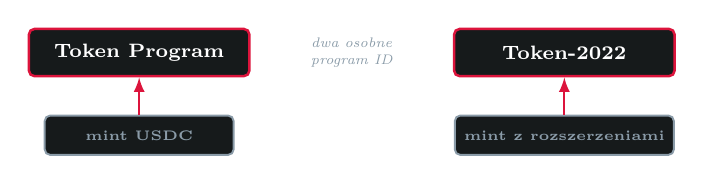
\begin{tikzpicture}[
        every node/.style={font=\scriptsize\bfseries, align=center},
        box/.style={
          draw=stplred, line width=0.9pt,
          fill=stplcard, text=stplwhite,
          rounded corners=2pt,
          minimum width=2.8cm, minimum height=0.6cm, align=center,
        },
        small/.style={
          draw=stplmuted, line width=0.7pt,
          fill=stplcard, text=stplmuted,
          rounded corners=2pt,
          minimum width=2.4cm, minimum height=0.5cm, align=center,
          font=\tiny\bfseries,
        },
        arr/.style={-latex, draw=stplred, line width=0.8pt},
        lbl/.style={font=\tiny\itshape, text=stplmuted},
      ]
      \node[box] (spl) at (0,   0.6) {Token Program};
      \node[box] (t22) at (5.4, 0.6) {Token-2022};

      \node[small] (m1) at (0,   -0.45) {mint USDC};
      \node[small] (m2) at (5.4, -0.45) {mint z rozszerzeniami};

      \draw[arr] (m1) -- (spl);
      \draw[arr] (m2) -- (t22);

      \node[lbl] at (2.7, 0.6) {dwa osobne\\program ID};
    \end{tikzpicture}
  \end{center}
  \vspace{-0.05cm}
  \begin{exampleblock}{Konsekwencja}
    Program obsługujący tokeny musi wiedzieć, do którego z dwóch programów
    kierować wywołanie --- i nie może tego zgadywać.
  \end{exampleblock}
\end{frame}

% 10. Interface --- code IS the slide (§4.3: code frame, no helper block)
\begin{frame}[fragile]{Interface}
  \begin{itemize}
    \item Konta tokenowe deklaruje się w Anchorze jak każde inne
    \item \texttt{Program<'info, Token>} przyjmuje dokładnie jeden program ID
    \item \texttt{Interface<'info, TokenInterface>} przyjmuje oba programy tokenowe
    \item Konta czyta się wtedy przez \texttt{InterfaceAccount}, nie \texttt{Account}
  \end{itemize}
  \begin{codeblock}{Konta tokenowe w strukturze instrukcji}
\begin{lstlisting}[style=reveal]
(*@\onslide<1->@*)#[derive(Accounts)]
(*@\onslide<1->@*)pub struct Lockup<'info> {
(*@\onslide<2->@*)    // tylko klasyczny SPL:
(*@\onslide<2->@*)    // pub token_program: Program<'info, Token>,
(*@\onslide<3->@*)    pub token_program: Interface<'info, TokenInterface>,
(*@\onslide<4->@*)    pub mint: InterfaceAccount<'info, Mint>,
(*@\onslide<4->@*)    pub vault: InterfaceAccount<'info, TokenAccount>,
(*@\onslide<1->@*)}
\end{lstlisting}
  \end{codeblock}
\end{frame}

% 11. Constraints tokenowe --- (alertblock: naming trap)
\begin{frame}[fragile]{Constraints tokenowe}
  \begin{itemize}
    \item \texttt{token::mint} --- konto tokenowe musi dotyczyć tego mintu
    \item \texttt{token::authority} --- kto podpisem autoryzuje operacje na koncie
    \item \texttt{token::token\_program} --- do którego programu konto należy
    \item Z Lekcji 6: Anchor sprawdza wszystkie trzy przed ciałem instrukcji
  \end{itemize}
  \vspace{0.15cm}
  \begin{alertblock}{Pułapka nazewnicza}
    Pole \texttt{owner} w koncie tokenowym to \textbf{authority}, a nie
    program będący właścicielem konta. Dwa pojęcia, jedno słowo.
  \end{alertblock}
\end{frame}

% ================================================================
\section{Podsumowanie}

\begin{frame}{Podsumowanie}
  \begin{enumerate}
    \item \textbf{Mint} opisuje walutę: podaż, \texttt{decimals}, prawo do dodruku
    \item \textbf{Token Account} trzyma saldo jednej pary właściciel--mint
    \item Portfel nie ma salda --- jest \textbf{authority} nad osobnym kontem
    \item \textbf{ATA} to adres wyliczony ze standardu; skarbiec wylicza program
    \item \textbf{Interface} pozwala obsłużyć klasyczny SPL i Token-2022 jednym kodem
  \end{enumerate}
  \vspace{0.2cm}
  \begin{exampleblock}{Efekt}
    Saldo tokena to nie liczba w portfelu, tylko konto z własnym adresem
    i własnym authority. To authority podpisuje każdy przelew.
  \end{exampleblock}
\end{frame}

% ================================================================
\begin{frame}[plain]
  \begin{center}
    \vfill
    {\Huge\bfseries\color{stplwhite} gn}
    \vfill
  \end{center}
\end{frame}

\end{document}
